\documentclass[xcolor=table]{cubeamer}
\usepackage{algorithm} % for using algorithm
\usepackage{algpseudocode} % for using algorithm
\usepackage{adjustbox} % for autoscaling of large table
\usepackage{pifont}%  % for checkmark and crossmark http://ctan.org/pkg/pifont
\usepackage{listings}
\usepackage{xcolor}

% setups
% \captionsetup[table]{skip=10pt}
\setbeamerfont{bibliography item}{size=\scriptsize}
\setbeamerfont{bibliography entry author}{size=\scriptsize}
\setbeamerfont{bibliography entry title}{size=\scriptsize}
\setbeamerfont{bibliography entry location}{size=\scriptsize}
\setbeamerfont{bibliography entry note}{size=\scriptsize}


\definecolor{codegreen}{rgb}{0,0.6,0}
\definecolor{codegray}{rgb}{0.5,0.5,0.5}
\definecolor{codepurple}{rgb}{0.58,0,0.82}
\definecolor{backcolour}{rgb}{0.95,0.95,0.92}

\lstdefinestyle{mystyle}{
    backgroundcolor=\color{backcolour},   
    commentstyle=\color{codegreen},
    keywordstyle=\color{magenta},
    numberstyle=\tiny\color{codegray},
    stringstyle=\color{codepurple},
    basicstyle=\ttfamily,
    breakatwhitespace=false,         
    breaklines=true,                 
    captionpos=b,                    
    keepspaces=true,                 
    numbers=left,                    
    numbersep=5pt,                  
    showspaces=false,                
    showstringspaces=false,
    showtabs=false,                  
    tabsize=2
}

\lstset{style=mystyle}

\title{LPython: Novel, Fast, Retargetable Python Compiler}
\subtitle{PyCon India 2023}

\author[Shaikh et al.]{
\texorpdfstring{\centering{Ubaid Shaikh, Ondřej Čertík, Brian Beckman, Gagandeep Singh, Thirumalai Shaktivel, Smit Lunagariya, Naman Gera, Pranav Goswami, Rohit Goswami, Dominic Poerio, Akshānsh Bhatt, Virendra Kabra, Anutosh Bhat, Luthfan Lubis, Dylon Thomas}}{Ubaid Shaikh, Ondřej Čertík, Brian Beckman, Gagandeep Singh, Thirumalai Shaktivel, Smit Lunagariya, Naman Gera, Pranav Goswami, Rohit Goswami, Dominic Poerio, Akshānsh Bhatt, Virendra Kabra, Anutosh Bhat, Luthfan Lubis, Dylon Thomas}
}

\date{September 30, 2023}

% \institute[GSI Technology]{GSI Technology}
% \copyrightnotice{Published by the American Institute of Aeronautics and Astronautics, Inc., with permission}

% defining commands
\newcommand{\cmark}{\ding{51}}%
\newcommand{\xmark}{\ding{55}}%

\begin{document}

\maketitle

% \cutoc

\section{Introduction}

% \begin{frame}{Brief about Speaker}
%     \begin{columns}
%         \begin{column}{0.7\textwidth}
%             \begin{itemize}
%                 \item Graduated from IIT Indore, CSE, 2022
%                 \item Compiler Developer at GSI Technology
%                 \item Working on LPython and LFortran Compilers
%                 \item In the past,
%                 \begin{itemize}
%                     \item interned at Development Bank of Singapore (DBS Bank)
%                     \item Google Summer of Code (GSoC) Fellow at Fortran-Lang Organization
%                 \end{itemize}
%             \end{itemize}
%         \end{column}
%         \begin{column}{0.3\textwidth}
%             \begin{figure}
%                 \centering
%                 \includegraphics[width=3.5cm]{images/my-photo.png}
%                 \caption{}
%             \end{figure}
%         \end{column}
%     \end{columns}
% \end{frame}
 
 \begin{frame}{Talk's agenda}
    \begin{itemize}
        \item Can we write a Python compiler that compiles fast and generates fast code?
        \item Online Demo
        \item Compiler stuff: 
        \begin{itemize}
            \item AST, ASR, Compiler Backends
            \item AOT, JIT, Interoperability with CPython
        \end{itemize}
        \item Summary
    \end{itemize}   
\end{frame}
\section{LPython}

\begin{frame}{LPython - Motivation}
    \begin{itemize}
        \item Python - long favoured for simplicity, intuitive syntax, productivity, ecosystem
        \item But inherently slow compared to other compiled langauges such as C and C++.
        \item LPython - Type Annotated Python Compiler for performance
        % \item Other compilers like Cython, Mojo, Numba, Pytorch exist. Why LPython?
        % \begin{itemize}
        %     \item Cython generates C code, but calls into Python for most Python features. Mojo is a superset, not compatible with CPython. Numba can't do ahead of time. PyTorch is only for AI stuff. 
        % \end{itemize}
        \item Most existing Python compilers focus on improving Python performance
        \item LPython aims to run Python at the maximum possible speed
    \end{itemize}
\end{frame}

\begin{frame}{LPython compared to C++}
    \begin{columns}
        \scalebox{.25}{
        \begin{column}{1.6\textwidth}
            \lstinputlisting[language=Python]{codes/dijkstra-code.py}
        \end{column}
        }
        \begin{column}{0.6\textwidth}
            \begin{figure}
                \centering
                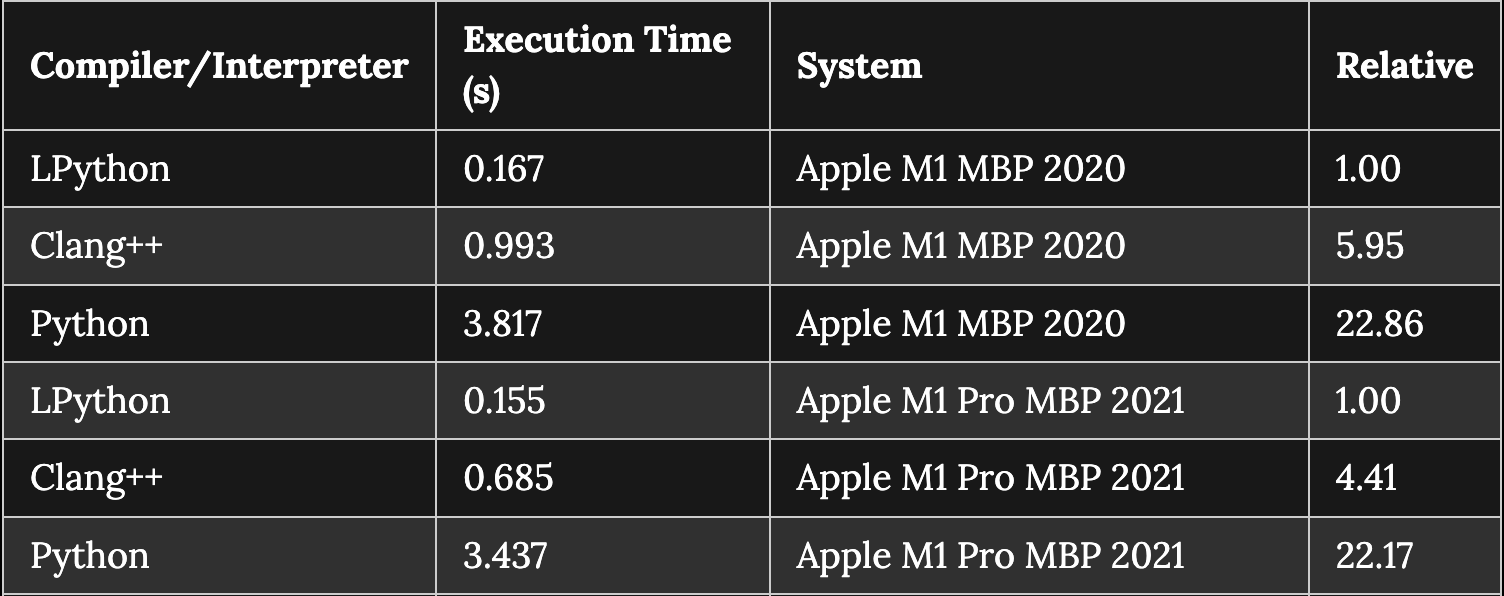
\includegraphics[width=7cm]{images/benchmark.png}
            \end{figure}
            \scriptsize \centering Note that the following optimization flags were used:
            \begin{figure}
                \centering
                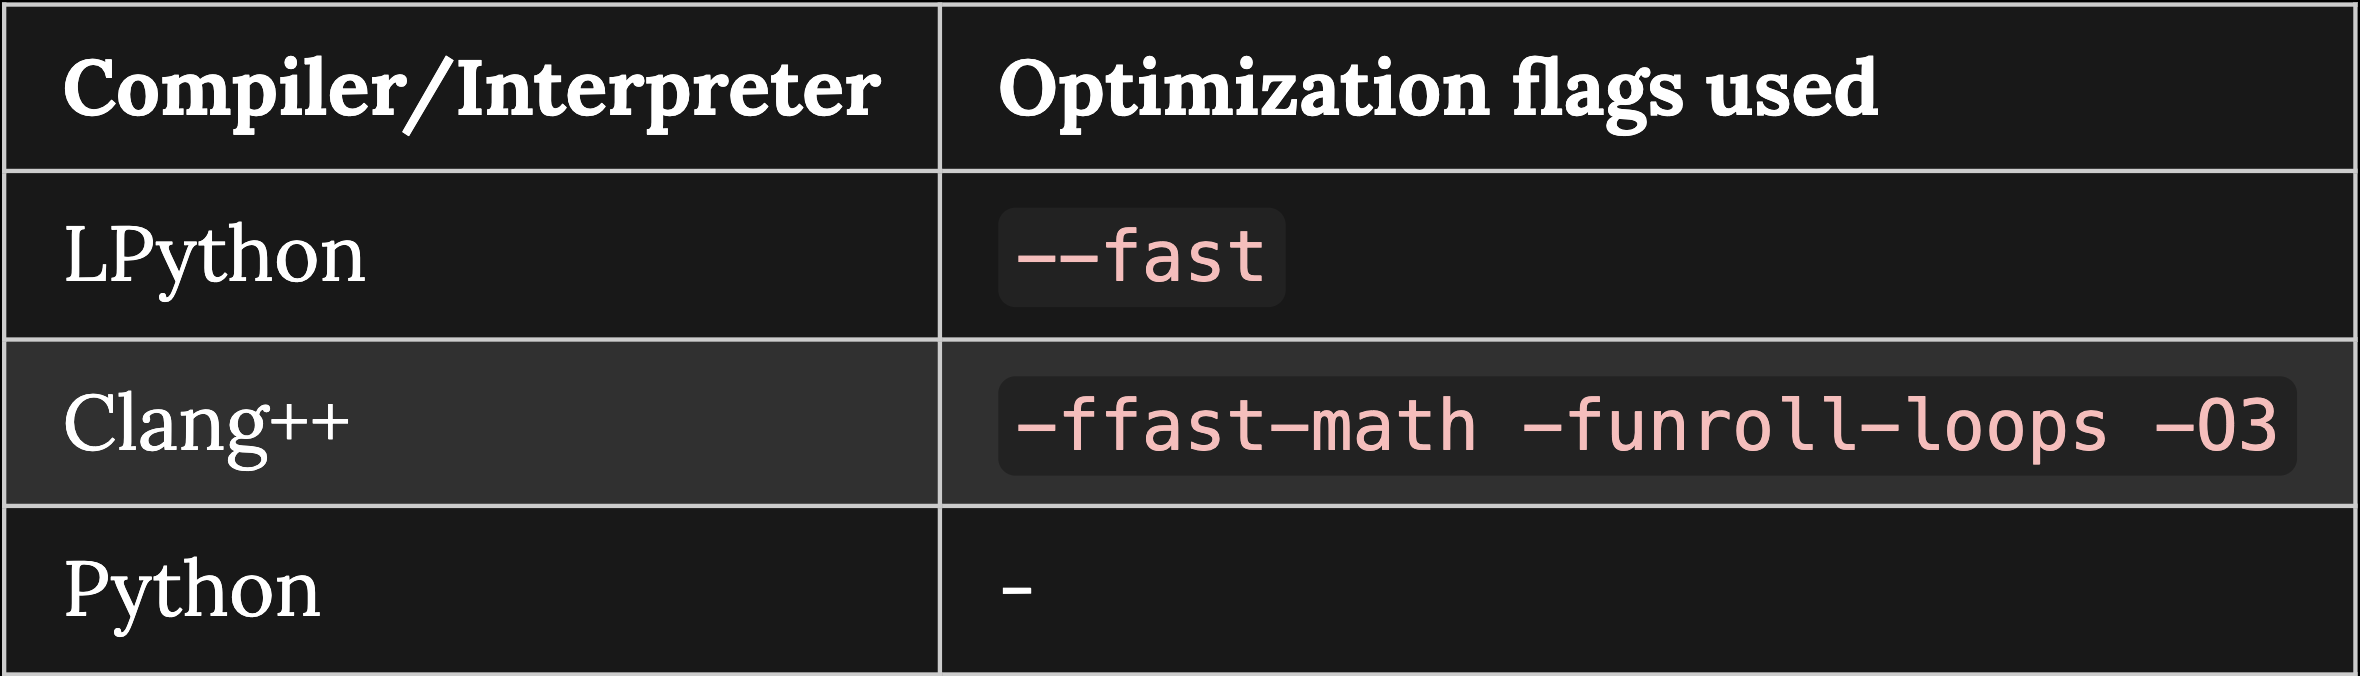
\includegraphics[width=5cm]{images/optimization-flags.png}
            \end{figure}
        \end{column}
    \end{columns}
    \scriptsize
    More Benchmarks at \href{https://lpython.org/blog/2023/07/lpython-novel-fast-retargetable-python-compiler/}{https://lpython.org/blog/2023/07/lpython-novel-fast-retargetable-python-compiler/}
\end{frame}

\begin{frame}{Star History}
    \begin{figure}
        \centering
        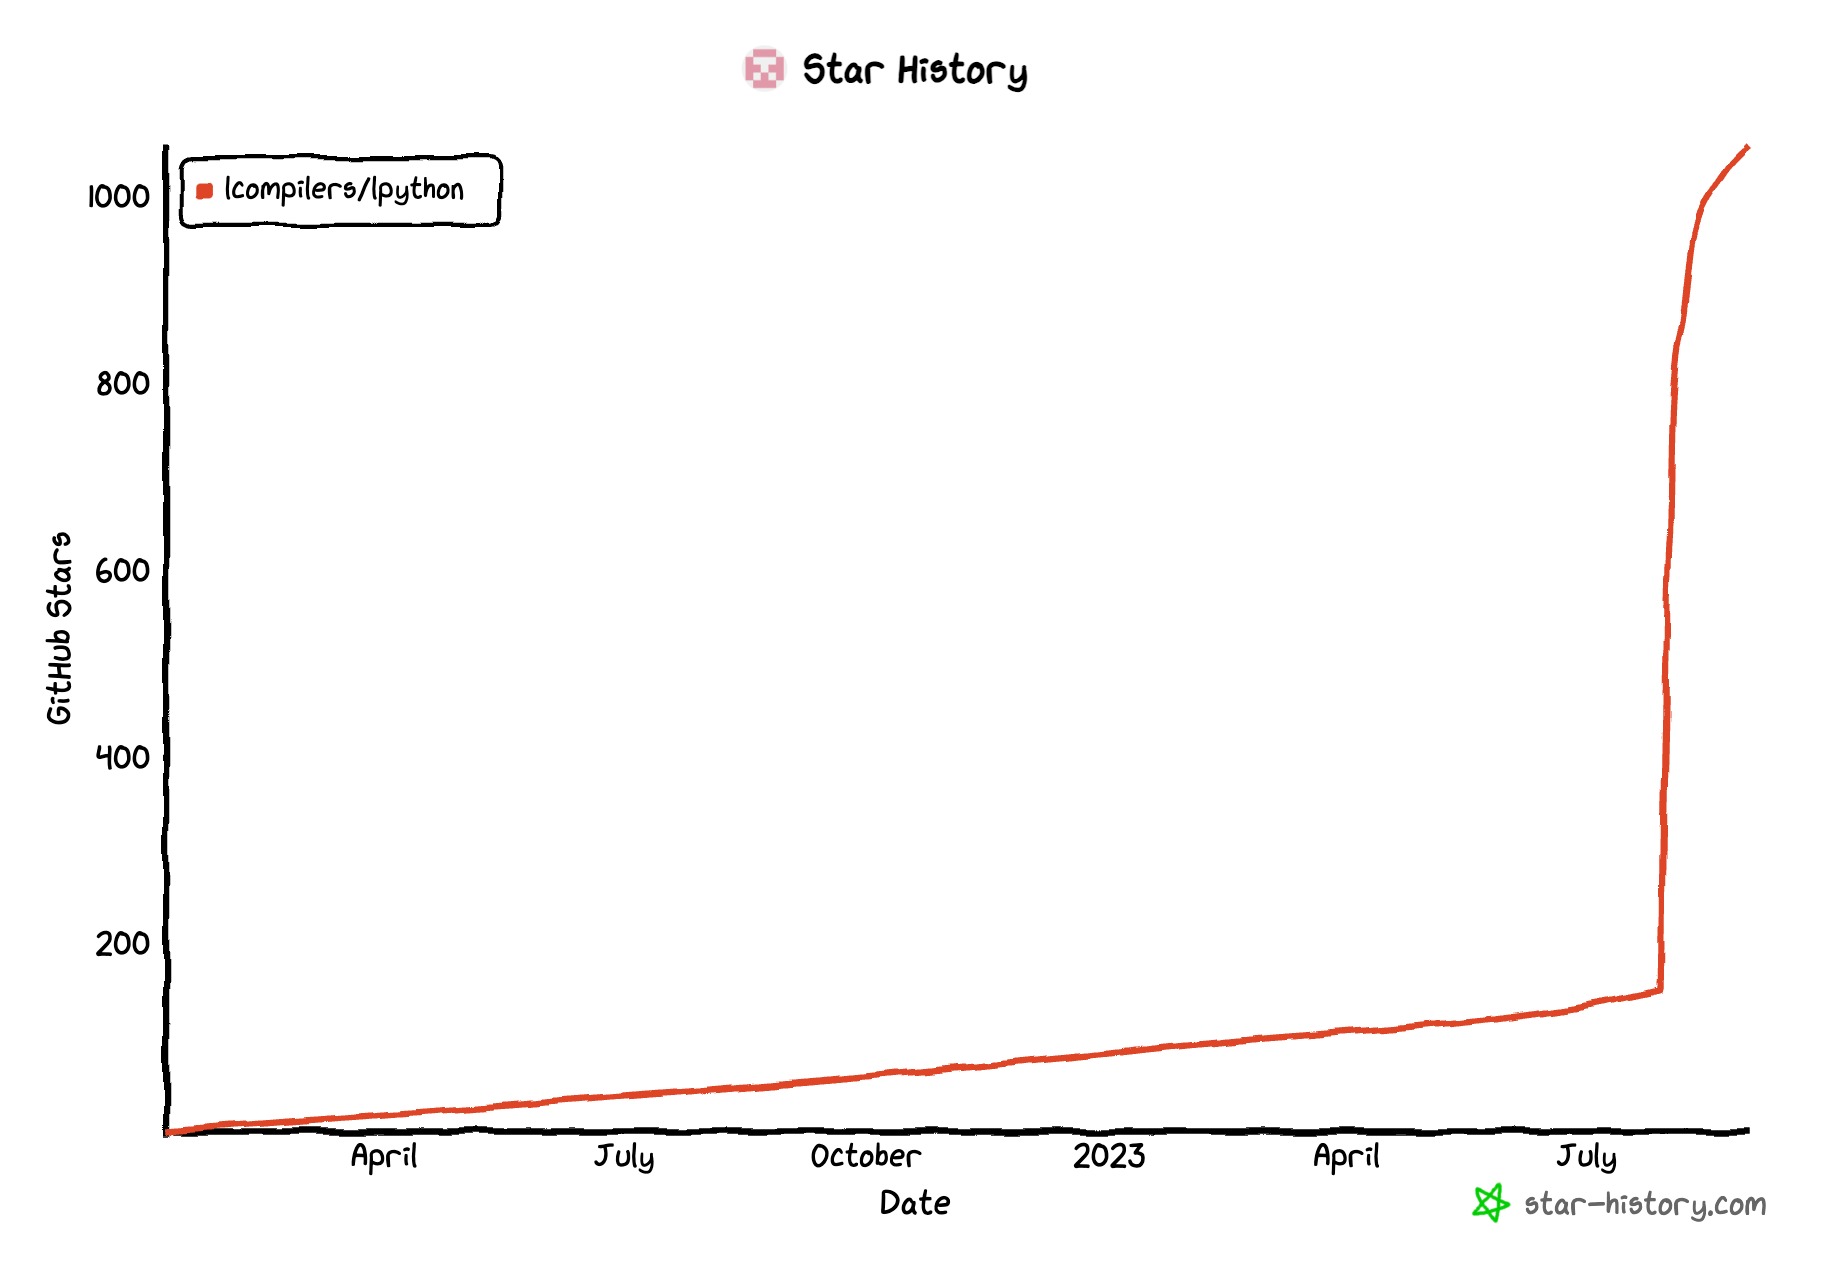
\includegraphics[width=8cm]{images/star-history.png}
        \caption{Spike in star count when we released LPython alpha}
    \end{figure}   
\end{frame}

\begin{frame}{LPython}
    \begin{columns}
        \begin{column}{0.5\textwidth}
            \scriptsize
            \lstinputlisting[language=Python]{codes/type-annotated-example.py}
            \centering Type annotated example code
        \end{column}
        \begin{column}{0.5\textwidth}
            \begin{itemize}
                \item Supports subset of CPython
                \item Requires types (annotations)
                \item If LPython compiles and runs, it will run in CPython
                \item Never slower than C and C++
                \begin{itemize}
                    \item \tiny{If you find an example where it is slower, it is a bug and we request you to report it to us.}
                \end{itemize}
                \item Several backends: LLVM, C, C++, WASM, X64 (via WASM)
            \end{itemize}
        \end{column}
    \end{columns}
\end{frame}

\section{Online Demo (dev.lpython.org)}
\section{LPython Annotation Types}

\begin{frame}{LPython - Annotation Types}
    \begin{columns}
        \begin{column}{0.5\textwidth}
            \tiny
            \lstinputlisting[language=Python]{codes/lpython-annotations-1.py}
            \centering Annotations for variables
        \end{column}
        \begin{column}{0.5\textwidth}
            \begin{itemize}
                \item Supports Integer types - \texttt{i8}, \texttt{i16}, \texttt{i32}, \texttt{i64}
                \item Similarly unsigned integers
                \item Floating points and Complex numbers
                \item Constant variables that need initialization value at the time of declaration
                \item Aggregate types like \texttt{list}, \texttt{tuple}, \texttt{classes} and more
            \end{itemize}
        \end{column}
    \end{columns}
\end{frame}

\begin{frame}{LPython - Annotation Types}
    \begin{columns}
        \begin{column}{0.5\textwidth}
            \tiny
            \lstinputlisting[language=Python]{codes/lpython-annotations-2.py}
            \centering Annotations, decorators for functions
        \end{column}
        \begin{column}{0.5\textwidth}
            \begin{itemize}
                \item Annotate function parameters and return types
                \item Supports generics.
                \begin{itemize}
                    \item \scriptsize{We have ongoing work on it.}
                \end{itemize}
                \item Supports specifying intents (In, InOut, Out) for function parameters.
                \begin{itemize}
                    \item \scriptsize{\texttt{In} - variable cannot be modified}
                    \item \scriptsize{\texttt{InOut} - variable can be modified}
                \end{itemize}
                \item \texttt{@lpython} and \texttt{@pythoncall} decorators
                \begin{itemize}
                    \item \scriptsize \texttt{lpython} calling from CPython into LPython 
                    \item \scriptsize \texttt{pythoncall} calling from LPython into CPython
                \end{itemize}
            \end{itemize}
        \end{column}
    \end{columns}
\end{frame}
\section{Abstract Syntax Tree and Abstract Semantic Representation}

\begin{frame}{Abstract Syntax Tree (AST)}
    \begin{columns}
        \begin{column}{0.5\textwidth}
            \lstinputlisting[language=Python]{codes/simple-example.py}
            \centering Example
        \end{column}
        \begin{column}{0.5\textwidth}
            \begin{figure}
                \centering
                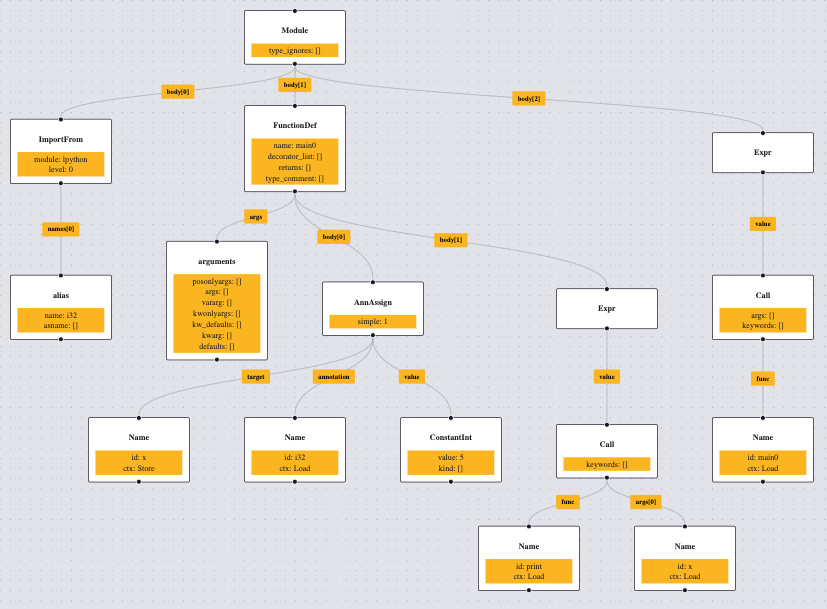
\includegraphics[width=7cm]{images/ast.png}
                \caption{AST}
            \end{figure}
        \end{column}
    \end{columns}
\end{frame}

\begin{frame}{Abstract Semantic Representation (ASR)}
    \begin{columns}
        \begin{column}{0.5\textwidth}
            \begin{figure}
                \centering
                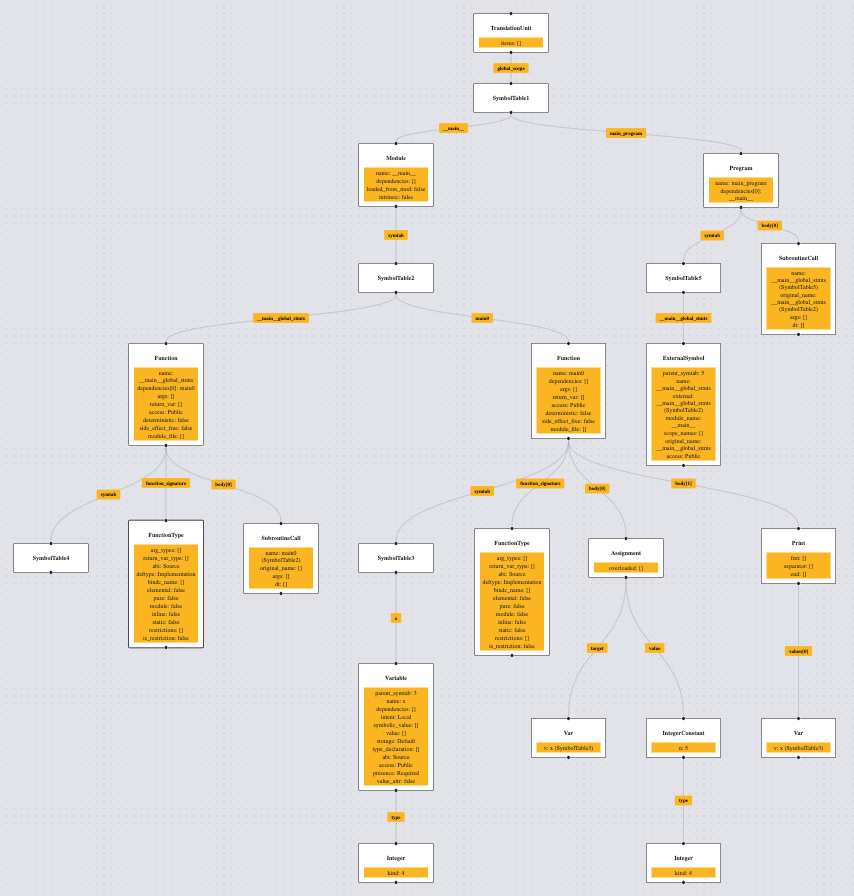
\includegraphics[width=5cm]{images/asr.png}
                \caption{ASR}
        \end{figure}
        \end{column}
        \begin{column}{0.5\textwidth}
            \begin{itemize}
                \item Independent of the frontends and backends
                \item As high level as possible, but faithful to the surface language
                \item ASR $\rightarrow$ ASR passes
                \begin{itemize}
                    \item loop vectorize
                    \item dead code removal
                    \item inline function calls, etc.
                \end{itemize}
                \item ASR $\rightarrow$ Backends
            \end{itemize}
        \end{column}
    \end{columns}
\end{frame}
\section{Backends}

\begin{frame}{Backends}
    \begin{itemize}
        \item Can compile Type-annotated Python code to different targets
        \item Current supported backends
            \begin{itemize}
                \item LLVM
                \item C
                \item C++
                \item WASM
                \item X64 (via WASM)
            \end{itemize}
        \item Other backends planned (Python, Fortran, etc.)
    \end{itemize}
\end{frame}

\begin{frame}{LPython - Usage}
    \scriptsize
    \begin{itemize}
        \item \texttt{lpython main.py --show-tokens}
        \item \texttt{lpython main.py --show-ast}
        \item \texttt{lpython main.py --show-ast --tree}
        \item \texttt{lpython main.py --show-ast --json}
        \item \texttt{lpython main.py --show-ast --visualize} (earlier image)
       \item \texttt{lpython main.py --show-asr}
        \item \texttt{lpython main.py --show-asr --tree}
        \item \texttt{lpython main.py --show-asr --json}
        \item \texttt{lpython main.py --show-asr --visualize} (earlier image)
        \item \texttt{lpython main.py --show-c}
        \item \texttt{lpython main.py --show-cpp}
        \item \texttt{lpython main.py --show-wat}
        \item \texttt{lpython main.py --show-llvm}
        \item \texttt{lpython main.py} (by default LLVM backend is used. Compiles and runs the code)
        \item \texttt{lpython main.py --backend=llvm}
        \item \texttt{lpython main.py --backend=c}
        \item \texttt{lpython main.py --backend=wasm}
    \end{itemize}
\end{frame}

\begin{frame}{Example of compiling to C}
    \begin{columns}
        \begin{column}{0.5\textwidth}
            \tiny
            \lstinputlisting[language=Python]{codes/backend-example.py}
            \centering main.py
        \end{column}
        \begin{column}{0.5\textwidth}
            \texttt{\$ lpython main.py --show-c > main.c}
        \end{column}
    \end{columns}
\end{frame}

\begin{frame}{Example of compiling to C}
    \tiny
    \begin{columns}
        \begin{column}{0.5\textwidth}
            \lstinputlisting[language=C]{codes/backend-example-show-c-1.c}
        \end{column}
        \begin{column}{0.5\textwidth}
            \lstinputlisting[language=C]{codes/backend-example-show-c-2.c}
        \end{column}
    \end{columns}
\end{frame}
\section{Ahead of Time, Just In Time and CPython Interoperability}

\begin{frame}{Ahead of Time and Just In Time Compilation}
    \begin{columns}
        \begin{column}{0.5\textwidth}
            \centering AOT
        \end{column}
        \begin{column}{0.5\textwidth}
            \centering JIT
        \end{column}
    \end{columns}
    \begin{columns}
        \begin{column}{0.5\textwidth}
            \begin{itemize}
                \item By default compiles to LLVM when no backend is specified
                \item Other backends can be used by using \texttt{--backend=c}
                \item Supports C, C++, WASM, WASM\_X64 (which generates a lean binary)
            \end{itemize}
        \end{column}
        \begin{column}{0.5\textwidth}
            \begin{itemize}
                \item Just decorate Python function with \texttt{@lpython}
                \item Specifying the desired backend as, \texttt{@lpython(backend="c")} or \texttt{@lpython(backend="llvm")}
                \item Supports C Backend at the moment, LLVM and others planned
            \end{itemize}
        \end{column}
    \end{columns}
\end{frame}

\begin{frame}{Interoperability with CPython}
    \begin{columns}
        \begin{column}{0.5\textwidth}
            \centering email\_extractor.py (LPython)
        \end{column}
        \begin{column}{0.5\textwidth}
            \centering email\_extractor\_util.py (CPython)
        \end{column}
    \end{columns}
    \begin{columns}
        \begin{column}{0.5\textwidth}
            \tiny
            \lstinputlisting[language=Python]{codes/interop-1.py}
        \end{column}
        \begin{column}{0.5\textwidth}
            \tiny
            \lstinputlisting[language=Python]{codes/interop-2.py}
        \end{column}
    \end{columns}
    \begin{itemize}
        \item Supports C backend currently
        \scriptsize
        \lstinputlisting[language=Bash]{codes/bash-email-extractor-output.txt}
    \end{itemize}
\end{frame}
% \section{Benchmarks}
    
\begin{frame}{LPython compared to C++}
    \begin{columns}
        \scalebox{.25}{
        \begin{column}{1.6\textwidth}
            \lstinputlisting[language=Python]{codes/dijkstra-code.py}
        \end{column}
        }
        \begin{column}{0.6\textwidth}
            \begin{figure}
                \centering
                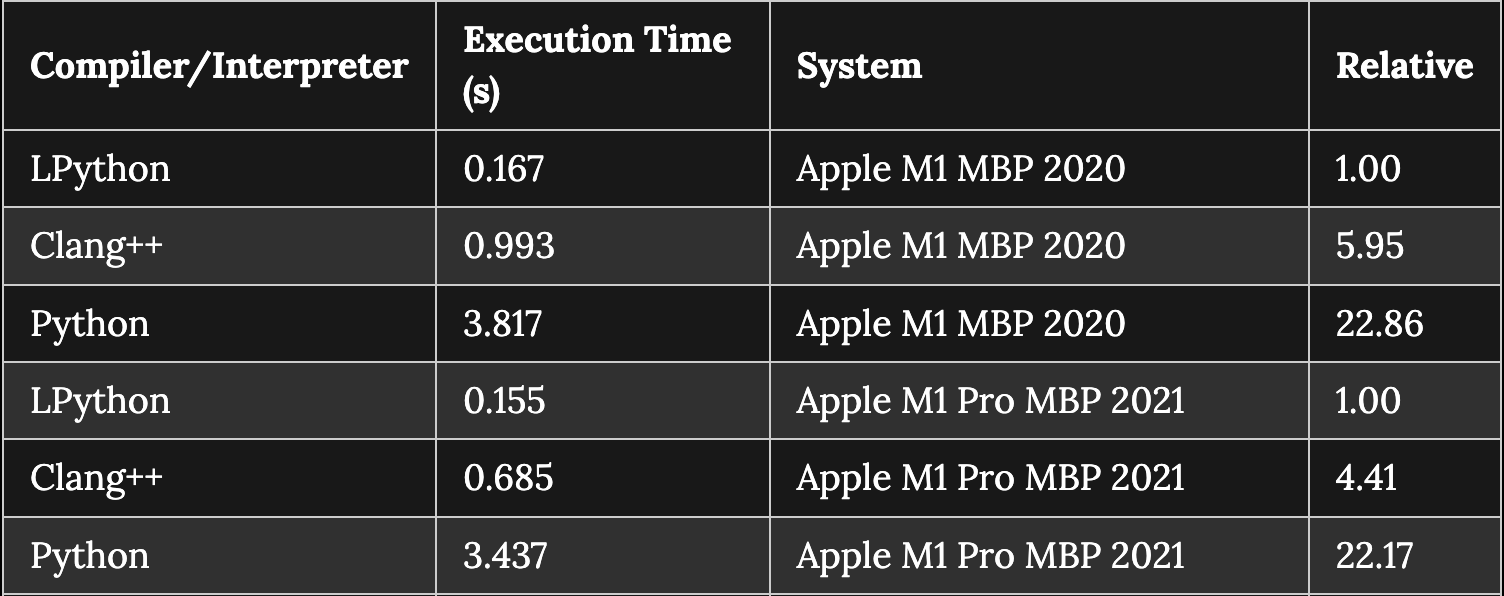
\includegraphics[width=7cm]{images/benchmark.png}
            \end{figure}
            \scriptsize \centering Note that the following optimization flags were used:
            \begin{figure}
                \centering
                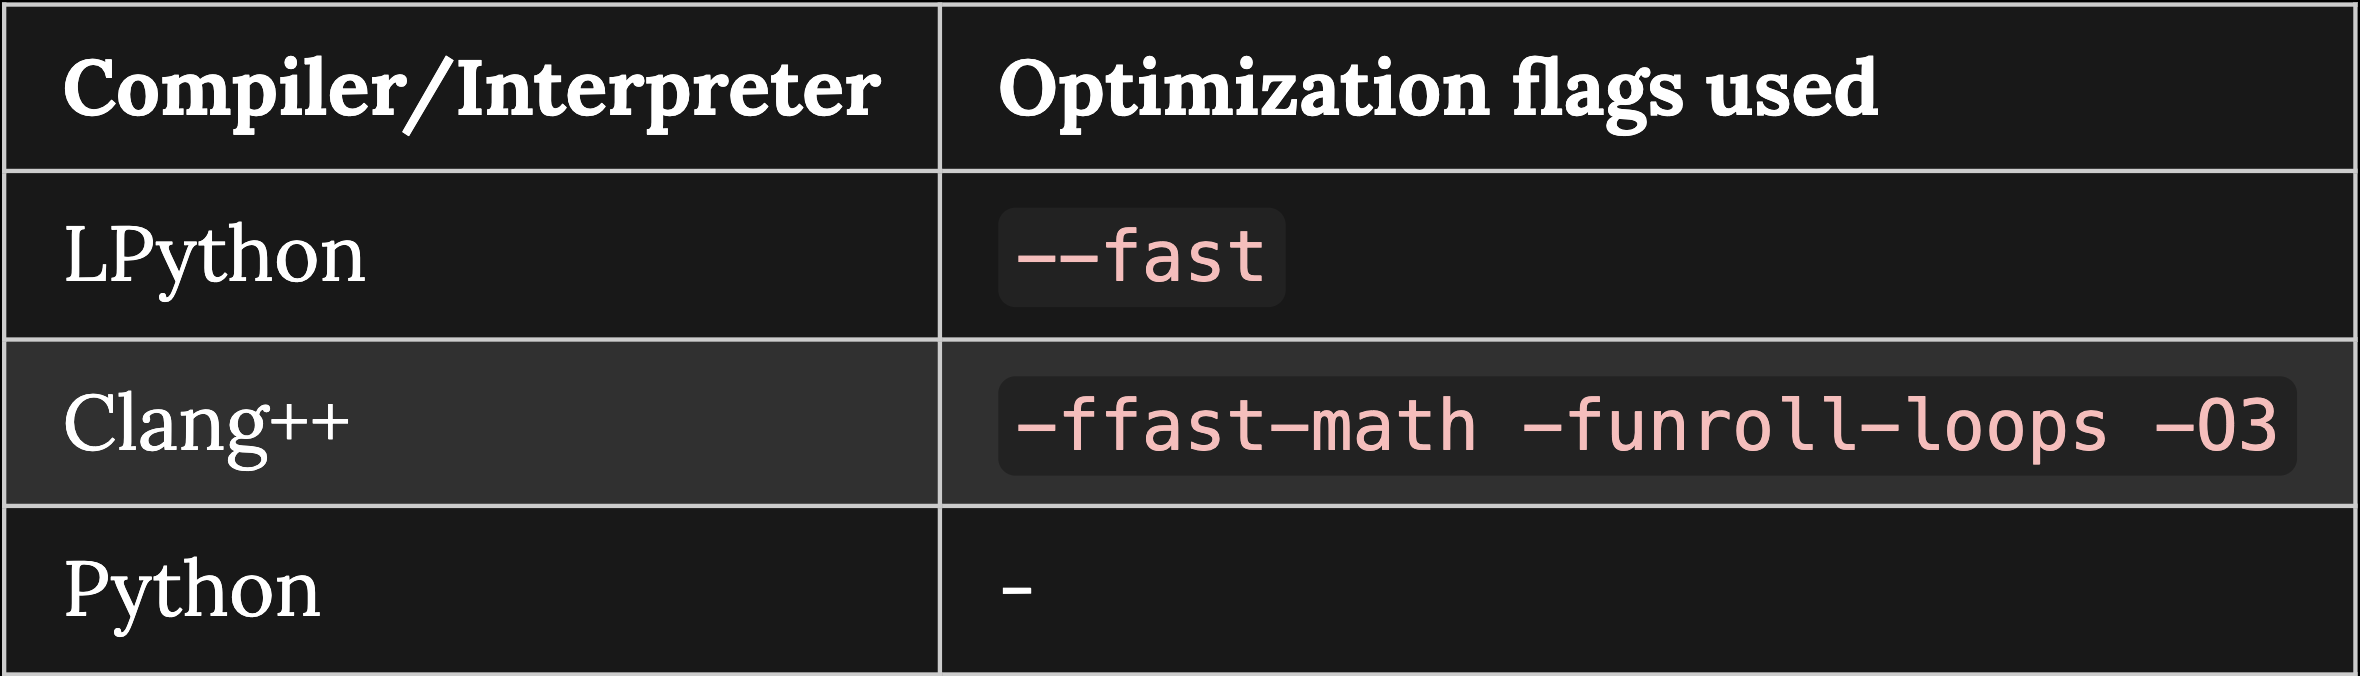
\includegraphics[width=5cm]{images/optimization-flags.png}
            \end{figure}
        \end{column}
    \end{columns}
    \scriptsize
    More Benchmarks at \href{https://lpython.org/blog/2023/07/lpython-novel-fast-retargetable-python-compiler/}{https://lpython.org/blog/2023/07/lpython-novel-fast-retargetable-python-compiler/}
\end{frame}
\section{Summary and Future Work}
    \begin{frame}{Summary}
        The compiler itself
        \begin{itemize}
            \item Implemented in C++
            \item Compiles in ~30s
            \item Fast compilation
            \item Fast runtime
            \item Custom AST/ASR tree representation and visitors
            \item Quickly loads and runs in a webpage
            \item \href{https://dev.lpython.org/}{https://dev.lpython.org/}
        \end{itemize}
    \end{frame}
    
    \begin{frame}{Future Work}
        \begin{itemize}
            \item More complete NumPy support (arrays)
            \item Strong support for structs and pointers (allows general
            programming)
            \item Make sure LPython is at least as fast as C++ for every simple
            benchmark (currently we have a few where we are slower)
            \item Make ‘@pythoncall‘ work with the LLVM backend
            \item Allow to extend LPython with custom hardware backends
            (GPU, APU, ...)
            \item Use LPython for bigger projects (ML, compilers, etc.)
            \item Optimizations
        \end{itemize}
    \end{frame}
\begin{frame}[standout]
    \Huge\textsc{Thank You!}

    \small If you're excited about the work we're doing on LPython, we invite you to come and contribute. We're always looking for new contributors to help us improve the project and make it more useful for everyone.
    \[\]
    \small
    Contact: shaikhubaid769@gmail.com

    GitHub: \href{https://github.com/Shaikh-Ubaid}{github.com/Shaikh-Ubaid}
\end{frame}


\end{document}
